\subsubsection*{Analysis}
\begin{tabular}{@{}l l}
\textbf{Scope}:&The AuctionHouse\textsuperscript{TM} automated administration system\\
\textbf{Level}:&User goal\\
\textbf{Primary Actor}:&Auctioneer\\
\textbf{Stakeholders and Interests}:&\begin{tabular}[t]{@{}l}Auctioneer: Wants to remove an item from the catalogue item list;
\\Tax Authorities: Wants to store the financial information of all items removed from\\ the catalogue item list due to being sold;
\\Owner: Same as tax authorities, plus wants to record the reason of deletion of each\\ individual item for administration purposes;
\\Viewer: Wants to see only non-removed items in the catalogue item list;  \end{tabular}\\
\textbf{Preconditions}:&\begin{tabular}[t]{@{}l}Actor is identified and authenticated.\\Actor is authorized to access this use case.\end{tabular}\\
\textbf{Postconditions}:&\begin{tabular}[t]{@{}l}The catalogue item list has been updated and does not contain the removed item.\\ Item is marked as deleted and the reason of deletion is recorded. If the item is \\deleted due to being sold it's financial information is recorded.  \end{tabular}\\
\textbf{Special requirements}:&\begin{tabular}[t]{@{}l}The item should be identifiable (perhaps with an unique identification number).\end{tabular}\\
\textbf{Frequency of occurence}:&Very frequent after each auction (once per month), otherwise rarely to even none at all.\\
\end{tabular}\\\\
\textsl{Main Success Scenario}
\begin{enumerate}[noitemsep]
	\item The user enters the deletion mode for items.
	\item The system displays a filterable list of all items from the individual item list that are not marked as deleted.
	\item The user filters the list using the following items characteristics:
	\begin{itemize}[noitemsep]
		\item The amount of the item available
		\item The type of item
		\item A description
		\item If the item possesses any antiquarian value
		\item A minimum price decided by the owner
		\item The date when brought in
		\item Name and address of the owner plus identification
		\item Planned auction date
		\item Distinguishing features
	\end{itemize}
	\item The user selects an item from the resultant filtered (shrinked) list.
	\item The systems prompts the user what is the reason of the deletion and records the answer.
	\item If the user answers "sold" - ask the user to specify the financial information for the item and record it, otherwise do nothing.
	\item The item is removed from catalogue item list.
	\item The user is notified about the succesfull deletion. 
\end{enumerate}
\textsl{Extensions}\\
\null\quad das
\\

\textsl{System Sequence Diagram}\\\\
\begin{figure}[H]
	\centering
	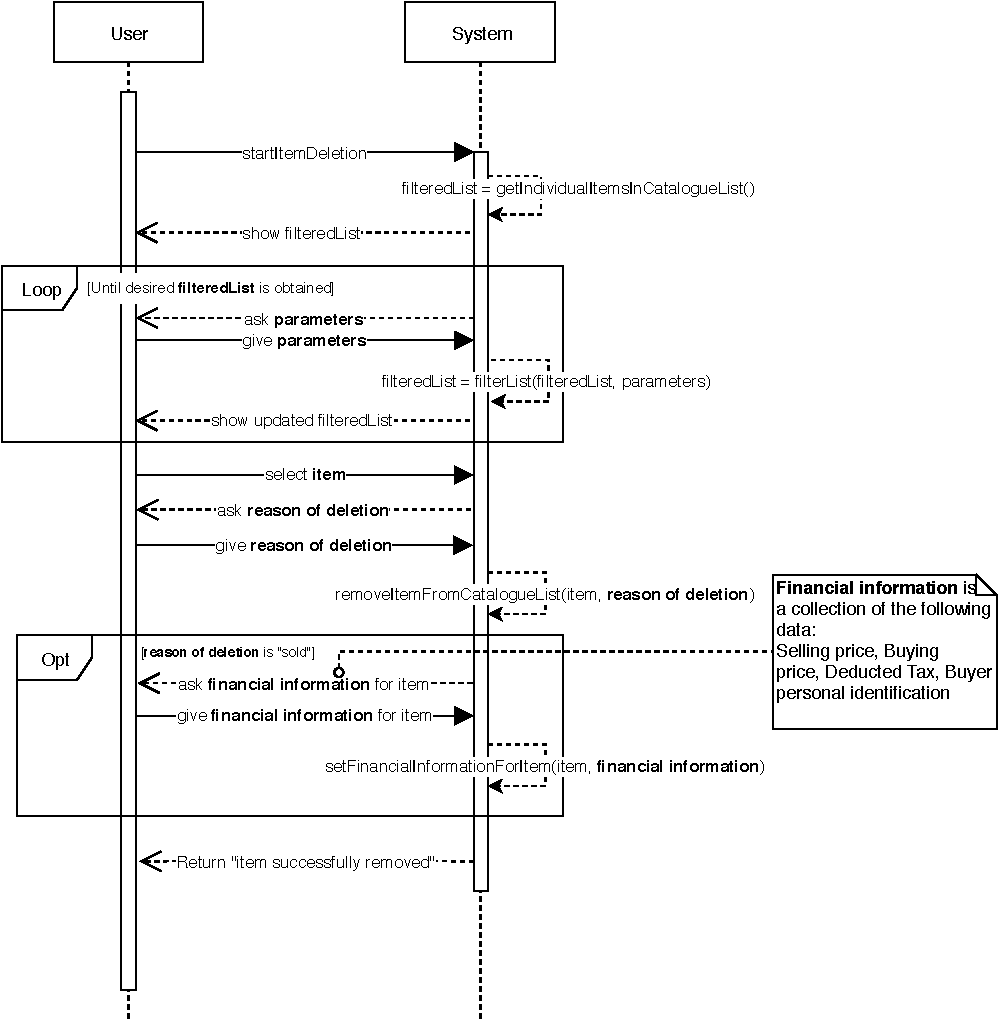
\includegraphics[scale=1]{uml/SD-bb-delete.pdf}
	\caption*{Interactions displayed in a System Sequence Diagram defined by the MSS and its extensions in blackbox format.}
\end{figure}